% !TEX TS-program = xelatex
% !TEX encoding = UTF-8 Unicode

% beamer loads xcolor itself, so options must be passed before the class is
% loaded -- otherwise we get an "Option clash for package xcolor".
\PassOptionsToPackage{x11names,dvipsnames}{xcolor}

\documentclass[10pt, compress]{beamer}

\usepackage{xcolor}

\usetheme{glasgow}
\usepackage{graphicx}
\graphicspath{{./}}
\usepackage{tikz}
\usepackage[normalem]{ulem} 
\newcommand\redout{\bgroup\markoverwith
{\textcolor{red}{\rule[0.5ex]{2pt}{0.8pt}}}\ULon}

\usetikzlibrary{arrows}
\usetikzlibrary{cd}
\usetikzlibrary{positioning}
\usetikzlibrary{fadings}
\usetikzlibrary{decorations.pathreplacing}
\usetikzlibrary{decorations.pathmorphing}
\tikzset{snake it/.style={decorate, decoration=snake}}

% styles for the matching examples
\tikzset{
  mvert/.style  = {circle, fill=university-slate, minimum size=5pt, inner sep=0pt},
  medge/.style  = {university-slate, line width=0.7pt},
  mmatch/.style = {university-pillarbox, line width=1.8pt},
}
\newcommand{\topline}
{%
  \tikz[remember picture,overlay] {%
    \draw[softGray] ([yshift=-1cm]current page.north west)
             -- ([yshift=-1cm,xshift=0.7\paperwidth]current page.north west);}
}

\usepackage{amsthm}

\newtheorem{question}{Question}
\newtheorem{conj}{Conjecture}


\usepackage{booktabs}
\usepackage[scale=2]{ccicons}

\usepgfplotslibrary{dateplot}


\title{Algorithms for temporal graph problems}
\subtitle{}
\date{\today}
\author{Jess Enright, Sam Hand, Laura Larios-Jones, Tom Davot, Jayakrishnan Madathil, Kitty Meeks, many others}
\institute{School of Computing Science, University of Glasgow}





\newcommand{\cc}{$c$-closed}
\newcommand{\card}[1]{\ensuremath{{\vert {#1} \vert }}}
\newcommand{\cl}{\ensuremath{\text{cl}}}

\newcommand{\lt}{\ensuremath{\Lambda}} %%%lifetime

\newcommand{\pngt}{\ensuremath{\Delta_0}} %%%parameter naught
\newcommand{\pone}{\ensuremath{\Delta_1}} %%%parameter one
\newcommand{\ptwo}{\ensuremath{\Delta_2}} %%%parameter two
\newcommand{\pcq}{\ensuremath{\Delta}} %%%parameter clique

\newcommand{\ppx}{\ensuremath{(\pcq, k + 1)}} %%%parameter plex 

\newcommand{\pdc}{\ensuremath{(\pcq, k)}} %%%parameter defective clique  

\newcommand{\pcod}{\ensuremath{(\pcq, generalizationd)}} %%%parameter co-degenerate

\newcommand{\tc}{\ensuremath{(\pngt, \pone, \ptwo, c)}} %%%temporal c

\newcommand{\tg}{\ensuremath{(\pngt, \pone, \ptwo, \gamma)}} %%%temporal gamma

\newcommand{\tp}{\ensuremath{(\pngt, \pone, \ptwo)}} %%%tuple of parameters

\newcommand{\nbdbound}{\ensuremath{c - 1 + 2\eta(\pcq - \pone)}}
\newcommand{\nbdboundplus}{\ensuremath{c - 1 + 2\eta(\pcq + 1 - \pone)}}

\newcommand{\weaknbdboundplus}{\ensuremath{c- 1 + 2\eta(\pcq + 1 - \pone)}}

% {\ensuremath{\Delta_1}} %%%parameter one
% \newcommand{\ptwo}{\ensuremath{\Delta_2}} %%%parameter two
% \newcommand{\pcq}{\ensuremath{\Delta}} %%%parameter clique


\newcommand{\mcbound}{\ensuremath{3 \cdot 2^{\nbdboundplus} \cdot n^2 \cdot \lt}} %%% maximal cliques bound

\newcommand{\weakmcbound}{\ensuremath{3 \cdot 2^{\weaknbdboundplus} \cdot n^2 \cdot \lt}} 

\newcommand{\mplexbound}{\ensuremath{4 \cdot 2^{\nbdboundplus} \cdot n^{\max\set{2k, k + 2}} \cdot \lt}}

\newcommand{\weakmplexbound}{\ensuremath{4 \cdot 2^{\weaknbdboundplus} \cdot n^{\max\set{2k, k + 2}} \cdot \lt}}

\newcommand{\mdcbound}{\ensuremath{4 \cdot 2^{\nbdboundplus} \cdot n^{k + 2} \cdot \lt}}

\newcommand{\weakmdcbound}{\ensuremath{4 \cdot 2^{\weaknbdboundplus} \cdot n^{k + 2} \cdot \lt}}

\newcommand{\ca}[1]{\ensuremath{\mathcal{#1} }}
\newcommand{\set}[1]{\ensuremath{\left\{ {#1} \right\}}}

\begin{document}

\maketitle

\begin{frame}
The Plan
\begin{itemize}
\item Temporal graphs
\item ... and what I'm not talking about
\item ... and why I got interested in them
\item Problems on temporal graphs
\item A crash course in parameterised algorithmics
\item Parameters for temporal graphs
\end{itemize}
% \item Temporal graphs and parameterised algorithms
% \item An example motivating problem
% \item Convenient temporal locality notion\textcolor{red}{s}
% \item Solving these convenient problems using VIM and TIM decompositions
% \end{itemize}
\end{frame}

\begin{frame}{Temporal graphs}
Here, a temporal graph is a graph with a function that specifies when an edge is active:  $\mathcal{G} = (G, \lambda)$


\begin{columns}[c]
% create the column with the first image, that occupies
% half of the slide
    \begin{column}{.5\textwidth}
    \begin{figure}
        \centering
            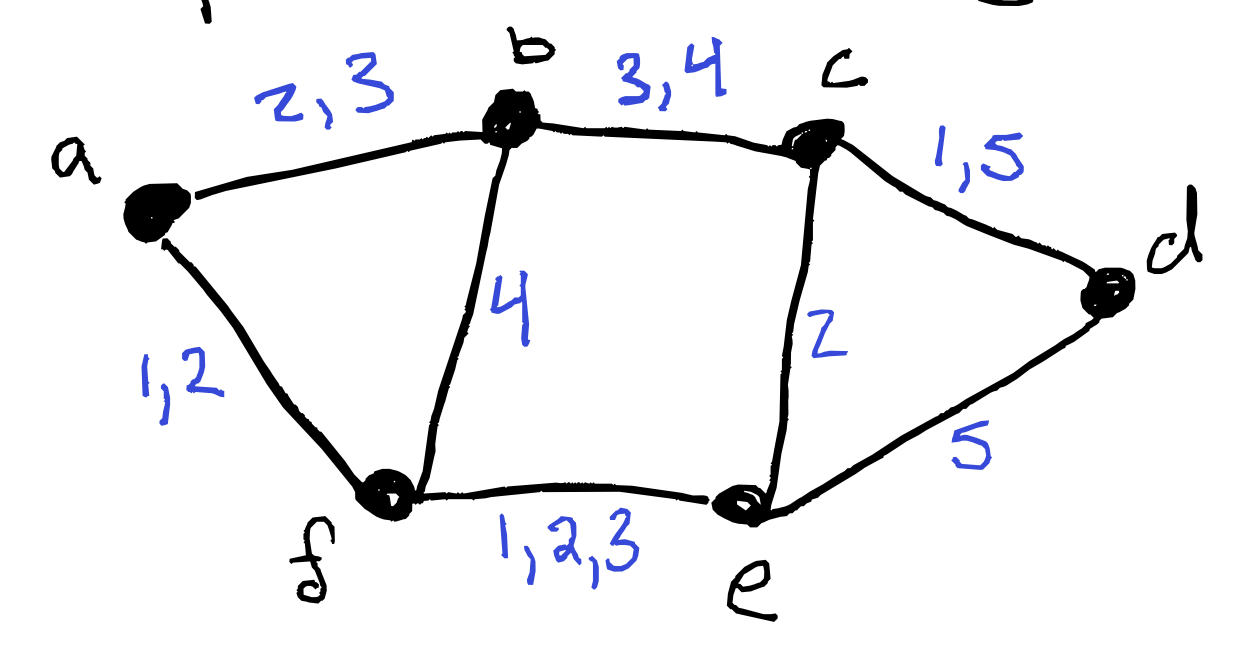
\includegraphics[width=1\linewidth]{temporal-graph.png}
        \end{figure}    
    \end{column}
% create the column with the second image, that also
% occupies half of the slide
    \begin{column}{.2\textwidth}
    \begin{figure}
        \centering
            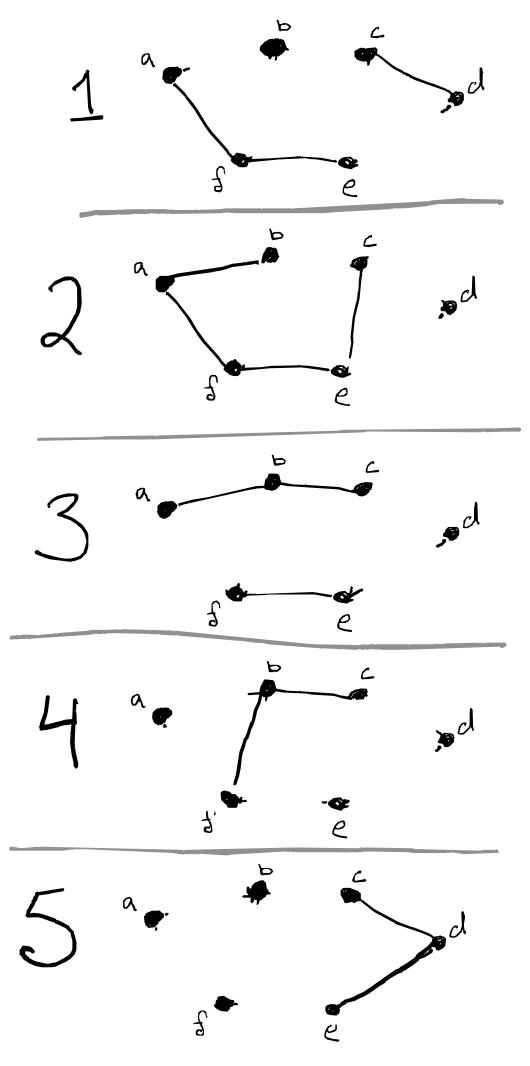
\includegraphics[width=1\linewidth]{snapshots-view.png}
        \end{figure}
    \end{column}

\end{columns}

A few important ideas:
 \begin{itemize}
 \item The underlying graph, or footprint
 \item lifetime
% \item active intervals
 \end{itemize}

\end{frame}

\begin{frame}{Everything is harder on temporal graphs}

\only<1>{
 \textsc{Maximum Temporal Matching}\\
 \textit{Input:} A temporal graph $(G,\lambda)$ and $\Delta \in \mathbb{N}$.\\
 \textit{Question:} What is the maximum cardinality of a set of time-edges $\mathcal{E}$ such that, for every pair of time-edges $(wx,t_1)$ and $(yz,t_2)$ in $\mathcal{E}$, either $\{w,x\} \cap \{y,z\} = \emptyset$ or $|t_1 - t_2| \ge \Delta$.

 \medskip

\begin{columns}[t]
\begin{column}{0.46\textwidth}
\centering
\begin{tikzpicture}
  \node[mvert] (a) at (0,0) {};
  \node[mvert] (b) at (1.3,0) {};
  \node[mvert] (c) at (2.6,0) {};
  \node[mvert] (d) at (3.9,0) {};
  \node[below=3pt of a] {$a$};
  \node[below=3pt of b] {$b$};
  \node[below=3pt of c] {$c$};
  \node[below=3pt of d] {$d$};
  \draw[mmatch] (a) -- (b);
  \draw[medge]  (b) -- (c);
  \draw[mmatch] (c) -- (d);
  \node[above=10pt] at (1.95,0) {\phantom{$\{2,5\}$}};
\end{tikzpicture}

\smallskip

{\small A maximum matching in the footprint: \textbf{2 edges}}
\end{column}
\begin{column}{0.46\textwidth}
\centering
\begin{tikzpicture}
  \node[mvert] (a) at (0,0) {};
  \node[mvert] (b) at (1.3,0) {};
  \node[mvert] (c) at (2.6,0) {};
  \node[mvert] (d) at (3.9,0) {};
  \node[below=3pt of a] {$a$};
  \node[below=3pt of b] {$b$};
  \node[below=3pt of c] {$c$};
  \node[below=3pt of d] {$d$};
  \draw[mmatch] (a) -- (b);
  \draw[mmatch] (b) -- (c);
  \draw[mmatch] (c) -- (d);
  \node[above=2pt] at (0.65,0) {\small $\{2,\textcolor{university-pillarbox}{\mathbf{5}}\}$};
  \node[above=2pt] at (1.95,0) {\small $\{\textcolor{university-pillarbox}{\mathbf{3}}\}$};
  \node[above=2pt] at (3.25,0) {\small $\{\textcolor{university-pillarbox}{\mathbf{1}}\}$};
\end{tikzpicture}

\smallskip

{\small A maximum $\Delta$-temporal matching, $\Delta = 2$: \textbf{3 time-edges}}
\end{column}
\end{columns}

\medskip

{\small $b$ and $c$ are each matched twice, because their two appearances are $\Delta$ apart. But we had to pick the \emph{right} appearance of $ab$: taking $(ab,2)$ instead of $(ab,5)$ would clash with $(bc,3)$.}
 }



 \only<2>{
 \textsc{Eulerian Circuit} (the static problem)\\
 \textit{Input:} A connected graph $G$.\\
 \textit{Question:} Is there a closed walk using every edge exactly once?

 \medskip

 \textbf{Euler, 1736:} yes iff every vertex has \textbf{even degree}, and Hierholzer finds one in \textcolor{blue}{linear time}.

\begin{center}
\begin{tikzpicture}[scale=0.78,
  enum/.style={fill=white, inner sep=1pt, font=\scriptsize, text=university-pillarbox}]
  \node[mvert] (A) at (1.4, 2.6) {};
  \node[mvert] (B) at (0.0, 1.9) {};
  \node[mvert] (C) at (0.0, 0.5) {};
  \node[mvert] (D) at (1.4,-0.2) {};
  \node[mvert] (E) at (2.4, 3.1) {};
  \node[mvert] (F) at (4.2, 3.1) {};
  \node[mvert] (G) at (5.5, 2.6) {};
  \node[mvert] (H) at (3.6, 1.2) {};
  \node[mvert] (I) at (7.0, 1.3) {};
  \node[mvert] (J) at (5.6,-0.1) {};
  \draw[medge] (A) -- (B) node[enum, midway] {1};
  \draw[medge] (B) -- (C) node[enum, midway] {2};
  \draw[medge] (C) -- (D) node[enum, midway] {3};
  \draw[medge] (D) -- (A) node[enum, midway] {4};
  \draw[medge] (A) -- (E) node[enum, midway] {5};
  \draw[medge] (E) -- (F) node[enum, midway] {6};
  \draw[medge] (F) -- (G) node[enum, midway] {7};
  \draw[medge] (G) -- (H) node[enum, midway] {8};
  \draw[medge] (H) -- (D) node[enum, midway] {9};
  \draw[medge] (D) -- (J) node[enum, midway] {10};
  \draw[medge] (J) -- (G) node[enum, midway] {11};
  \draw[medge] (G) -- (I) node[enum, midway] {12};
  \draw[medge] (I) -- (J) node[enum, midway] {13};
  \draw[medge] (J) -- (H) node[enum, midway] {14};
  \draw[medge] (H) -- (A) node[enum, midway] {15};
\end{tikzpicture}
\end{center}

{\small Every degree here is $2$ or $4$: the numbers give one Eulerian circuit.}
 }

 \only<3>{
 \textsc{TempEuler}\\
 \textit{Input:} A temporal graph $(G,\lambda)$.\\
 \textit{Question:} Is there a closed temporal walk that contains every edge of $G$ exactly once?\\
 \vspace{0.5cm}

 \only<3>{Note: this is also called \textsc{Eulerian Trail} by Marino \& Silva.}

\only<3>{
\begin{center}
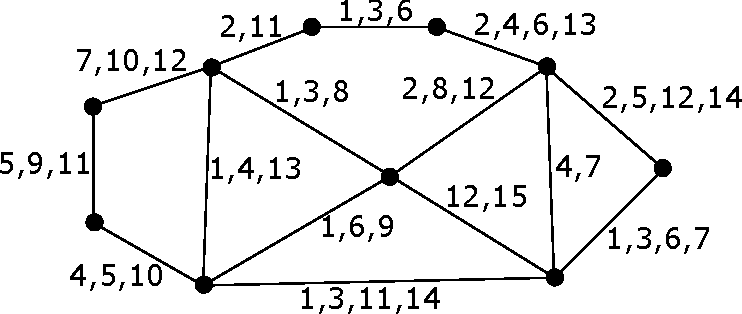
\includegraphics[width = 0.8 \linewidth]{TempEuler}
\end{center}
}

 }



\only<4-5>{
\textsc{StarExp}\\
\textit{Input:} A temporal graph $(S_n,\lambda)$, where $S_n$ is a star with $n$ leaves.\\
\textit{Question:} Does there exist a temporal walk, starting and ending at the centre of the star, that visits every vertex?


\begin{center}
\only<4>{%
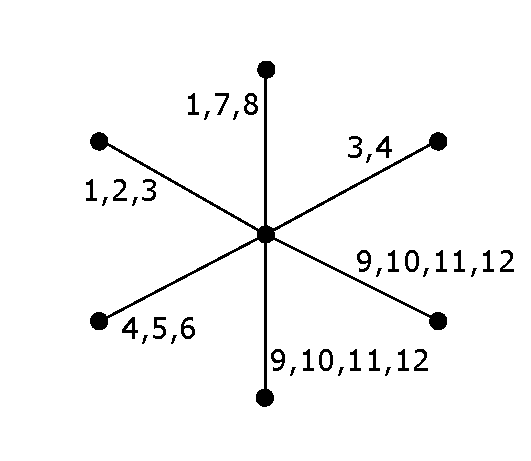
\includegraphics[width=0.5 \linewidth]{StarExp_Yes}%
}
\only<5>{%
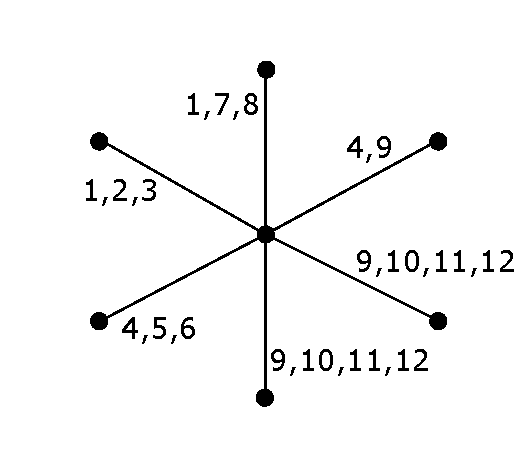
\includegraphics[width=0.5 \linewidth]{StarExp_No}%
}
\end{center}

}

\end{frame}

\begin{frame}{Problems on temporal graphs}
It's not just hard, but complicated - many problems on static graphs can be made temporal - but often in lots of different ways!

\bigskip

Example: Does there exist a \textbf{temporal clique} of size $k$?
\begin{itemize}
\item What counts for adjacency?
\begin{itemize}
\item \textbf{ever} adjacent?
\item \textbf{always} adjacent?
\item all adjacent at the \textbf{same time}
\item adjacent within some \textbf{time window} or with some \textbf{frequency}?
\end{itemize}
\bigskip
Depending on your definitions, the same vertex set could be both a temporal clique and a temporal independent set!

\end{itemize}
\end{frame}



\begin{frame}
So: why are you ruining your life (and the lives of your students) with these, Jess?

\bigskip

\bigskip


\bigskip

\begin{itemize}
\item Fun
\item \redout{Profit} Applications
\end{itemize}

\end{frame}

\begin{frame}{It all started with cows}
\begin{figure}
    \centering
    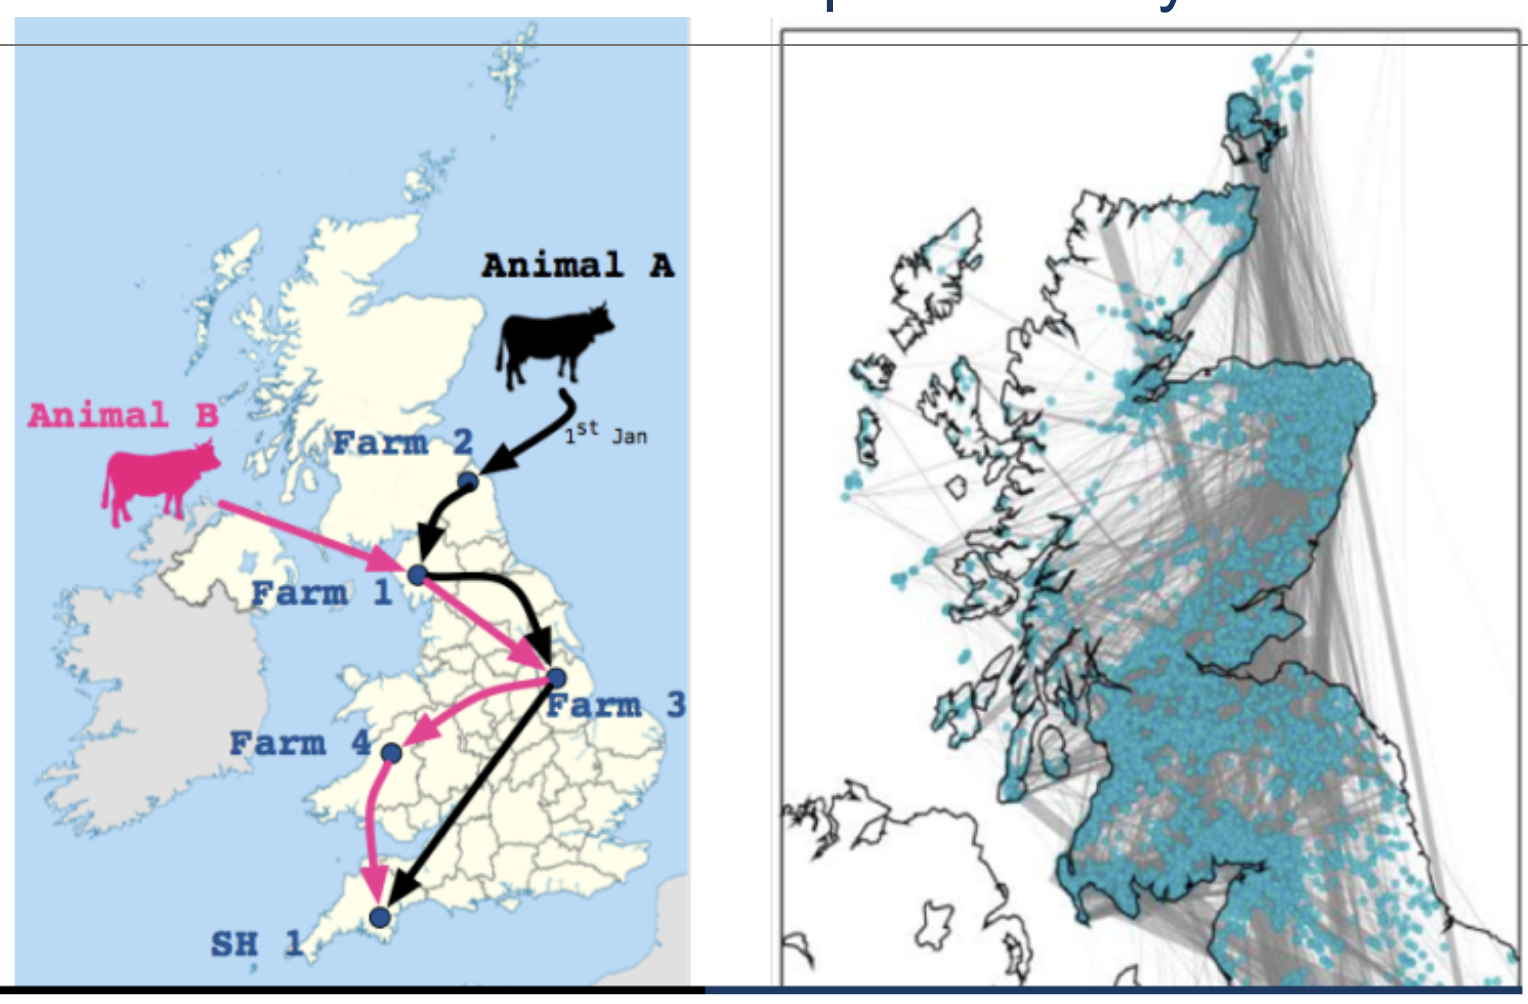
\includegraphics[width=1\linewidth]{cows.png}
\end{figure}
\end{frame}


\begin{frame}{Diseases and cattle travel only forward in time}
\begin{figure}
    \centering
    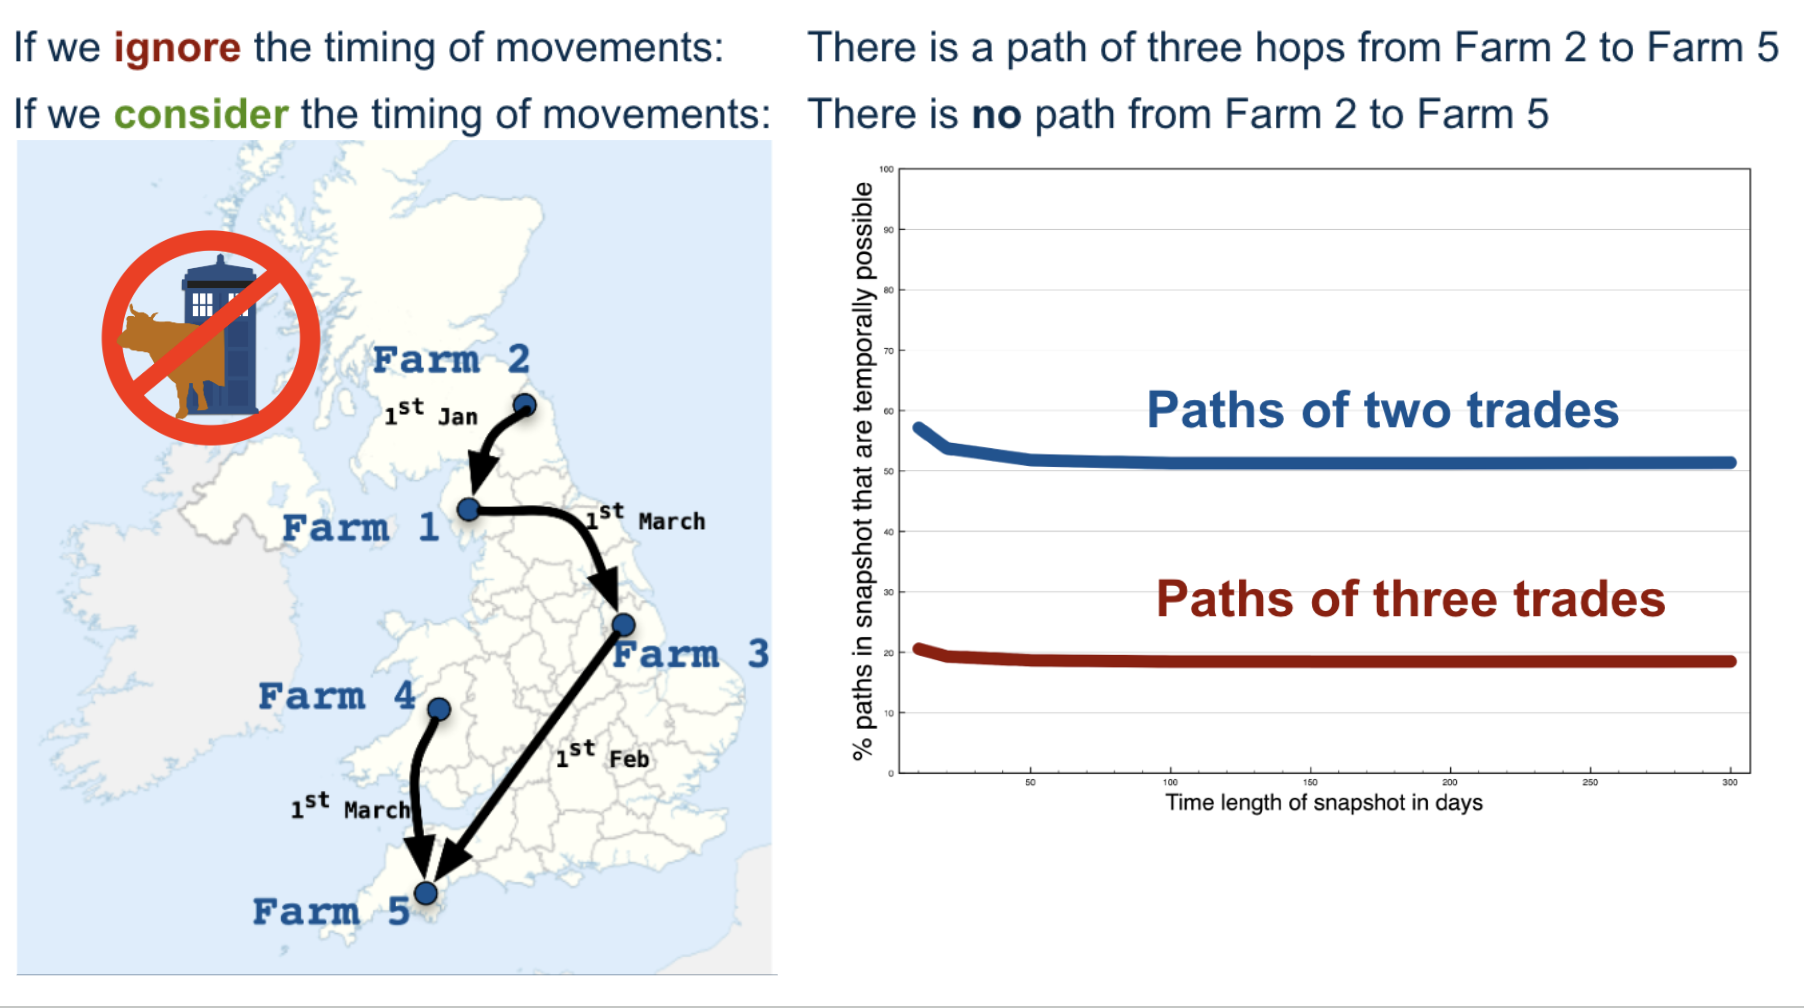
\includegraphics[width=1\linewidth]{cow-tardis.png}
\end{figure}
\end{frame}


\begin{frame}{Humans get diseases too}
\begin{figure}
    \centering
    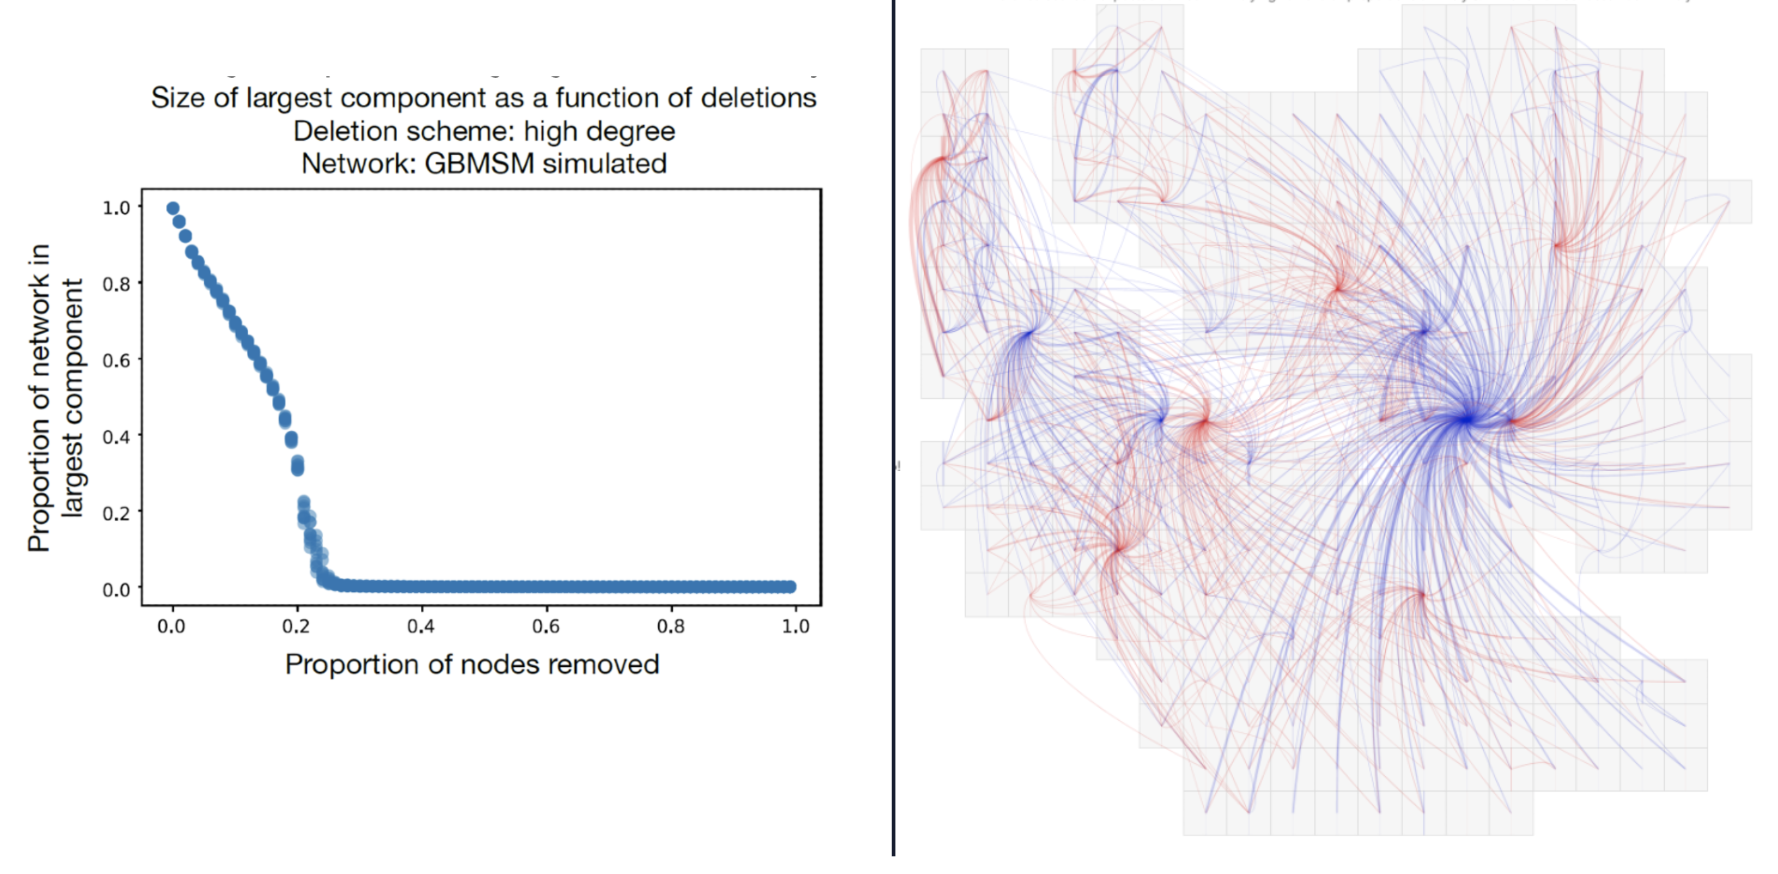
\includegraphics[width=0.8\linewidth]{human-epi-networks.png}
\end{figure}


\textbf{For both fun and profit we want to solve hard problems on temporal graphs}
\end{frame}


\begin{frame}{What do you do with an NP-hard problem?}
Suppose you want to solve one of these, and you want to solve it \textbf{exactly}.

\bigskip

\begin{itemize}
\item \redout{Give up}
\item Approximate it - but this may be impossible or insufficient
\item Heuristics - often excellent in practice, but no guarantees
\item Use a solver and accept an exponential in $n$ - fine until $n$ is the size of the cattle trade network
\end{itemize}

\bigskip

\textbf{Parameterised approach: work out what it is about your instances that makes them hard and tolerate an exponential related to that if it is small.}
\end{frame}


\begin{frame}{Parameterised algorithmics}
An instance is now a \textbf{pair} $(I, k)$: the input, plus a \emph{parameter} - some number we hope is small.

\bigskip

A problem is \textbf{\textcolor{blue}{fixed-parameter tractable (FPT)}} if it can be solved in time
\[
f(k) \cdot |I|^{\mathcal{O}(1)}
\]
for some computable $f$.  All of the badness is confined to $f$.

\bigskip

Compare \textbf{XP}: time $|I|^{f(k)}$, e.g. the $n^{k}$ you get by trying every $k$-subset.

\begin{center}
\begin{tabular}{l l}
\toprule
\textbf{Running time} & \textbf{$n = 10^4$, $k = 20$} \\
\midrule
$2^{k} \cdot n$ & about $10^{10}$ steps: fine \\
$n^{k}$ & about $10^{80}$ steps: not fine \\
\bottomrule
\end{tabular}
\end{center}
\end{frame}


\begin{frame}{The classic example}
\textsc{Vertex Cover}\\
\textit{Input:} A graph $G$ and an integer $k$.\\
\textit{Question:} Is there a set of at most $k$ vertices meeting every edge?

\bigskip

\textcolor{red}{NP-complete}, but: pick any edge $uv$; every cover contains $u$ or $v$.  Branch on which, and recurse with $k - 1$.

\bigskip

A search tree of depth $k$ and branching factor 2 gives $\mathcal{O}(2^{k}(n + m))$.

\bigskip

\textbf{So a 300-vertex network with a cover of size 20 is entirely reasonable, even though the problem is NP-complete.}
\end{frame}


\begin{frame}{Where does the parameter come from?}
Two broad flavours:

\begin{itemize}
\item \textbf{Solution size} - $k$ is the thing you are asked for: the size of the cover, the number of deletions, the length of the walk.
\item \textbf{Structural width} - $k$ measures how far the input is from something we can already handle: treewidth, vertex cover number, neighbourhood diversity, cliquewidth.
\end{itemize}

\bigskip

A parameter earns its keep if:
\begin{itemize}
\item it is genuinely \textbf{small} on the instances we care about,
\item we can \textbf{compute} (or approximate) it, and
\item bounding it actually \textbf{buys} us an algorithm.
\end{itemize}

\bigskip

\textbf{The first of these is an empirical question - we will come back to it at the end.}
\end{frame}



\begin{frame}{So we need parameterised approaches!}
How might we parameterise?
\begin{itemize}
    \item Restrict the underlying graph
    \item Restrict the temporal structure
    \item Restrict something else: e.g. solution size
\end{itemize}
\end{frame}

\begin{frame}{Restricting the underlying structure}

\begin{itemize}
\item \textsc{Maximum Temporal Matching} is \textbf{\textcolor{red}{NP-hard}} even when $G$ is a path (Mertzios, Molter, Niedermeier, Zamaraev \& Zschoche, 2020).
% \pause
\item \textsc{TempEuler} is \textbf{\textcolor{red}{NP-complete}} even if:
\begin{itemize}
\item each edge appears at only 2 times (Marino \& Silva, 2021);
\item each edge appears at only 3 times, and $G$ has feedback vertex number one (Bumpus \& Meeks, 2021);
\item each edge appears at only 4 times, and $G$ has vertex cover number 2 (Bumpus \& Meeks, 2021). 
\end{itemize}
% \pause
\item \textsc{StarExp} is solvable in \textbf{\textcolor{blue}{polynomial time}} if each edge appears at most 3 times (Akrida, Mertzios \& Spirakis, 2019), but \textbf{\textcolor{red}{NP-complete}}  if edges are allowed to appear 4 or more times (Bumpus \& Meeks, 2021); $G$ is always a tree of vertex-cover number 1.
\end{itemize}
\end{frame}




\begin{frame}{Temporal and underlying structure}

A sampler:
\begin{itemize}
    \item lifetime 
    \item lifetime plus underlying treewidth
    \item various temporal interpretations of treewidth
    \item timed vertex cover notions
    \item limiting the number of things you need to think about at a time
    \begin{itemize}
    \item edge interval membership width
    \item \textbf{vertex interval membership (VIM) width}
    \item TIM-width
    \end{itemize}
    \item Three nested ones that work for dense graphs:
    \begin{itemize}
    \item \textbf{temporal neighbourhood diversity}
    \item temporal modular width
    \item temporal cliquewidth
    \end{itemize}
    \item temporal clustering closedness
    
\end{itemize}



% Obvious temporal parameters:
% \begin{itemize}
% \pause
% \item lifetime 
% %sometimes gives tractability, but often for boring reasons e.g. TempEuler gives trivial no-instances.  Plenty of problems hard for constant lifetime.  More useful in combination with a structural parameter.
% \pause
% \item maximum number of times at which any edge appears
% %We saw examples where this is no help - StarExp and TempEuler
% \pause
% \item maximum number of edges appearing at any one time
% %StarExp is still NP-hard even if at most one edge appears at each time.
% \end{itemize}

% \pause
% \vspace{0.5cm}
% Parameters combining times and graph structure:
% \begin{itemize}
% \pause
% \item timed feedback vertex number %number of vertex appearances we must delete so that the *underlying* graph becomes cycle-free.  This is invariant under reordering the layers - in some sense it's about how often cycle-creating things appear
% \pause
% \item temporal feedback edge/connection number
% \pause
% \item several different temporal interpretations of treewidth
% \end{itemize}
% %always bounded if the underlying graph is a tree

\end{frame}


\begin{frame}{Temporal parameters}
A very restrictive temporal parameter:

\medskip
\redout{vertex-interval-membership} VIM width

\medskip
If a temporal graph has low VIM width that at every time most vertices have either finished being active or have not yet been active. 

\begin{columns}[c]
% create the column with the first image, that occupies
% half of the slide
    \begin{column}{.4\textwidth}
    \begin{figure}
        \centering
            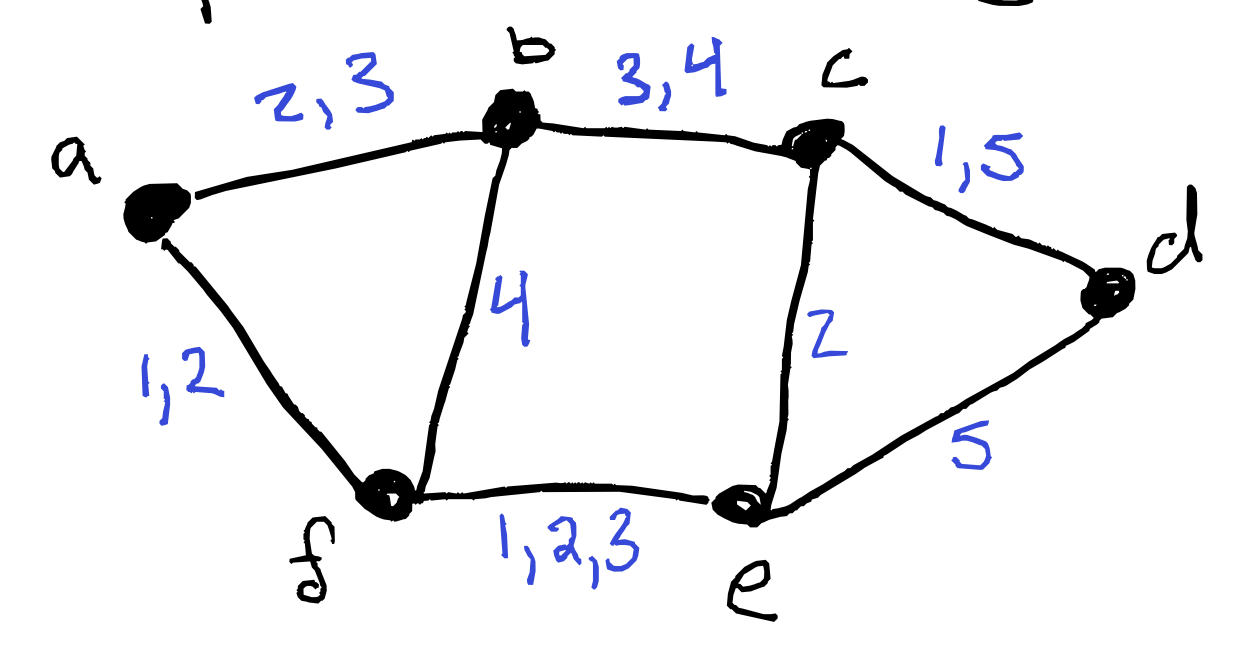
\includegraphics[width=1\linewidth]{temporal-graph.png}
        \end{figure}    
    \end{column}
% create the column with the second image, that also
% occupies half of the slide
    \begin{column}{.3\textwidth}
    \begin{figure}

            \centering
            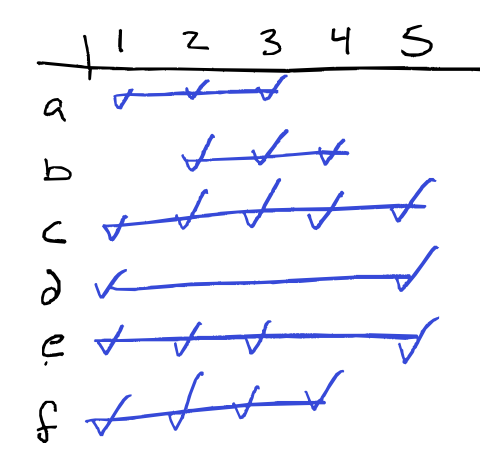
\includegraphics[width=1\linewidth]{vim-table.png}
        \end{figure}
    \end{column}


\end{columns}

Why do we care about this?  Sometimes we can devise algorithms that are $O(poly(n)\cdot f(\omega))$ where $\omega$ is our width

\end{frame}

\begin{frame}{VIM decomposition DPs}
How do VIM-decomposition dynamic programs work?
\begin{itemize}
\item make a series of bags, one for each time
\item starting at the beginning of time, consider all possibilities at each bag
\begin{itemize}
\item and be able to check that a possibility is consistent with one at the previous time, and is acceptable
\end{itemize}
\item get to the end of time, and see if you have solved the problem
\end{itemize}

\bigskip

\begin{figure}
    \centering
    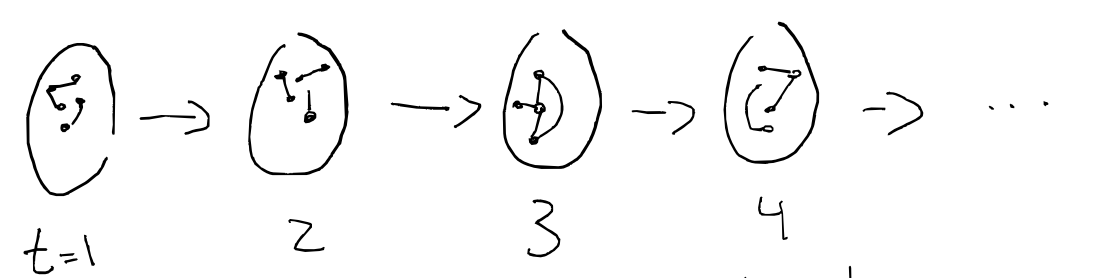
\includegraphics[width=0.75\linewidth]{vim-decomp.png}
\end{figure}

\end{frame}

\begin{frame}{Temporal graph problems}
Example: \textbf{Temporal Hamiltonian Path}
\begin{figure}
    \centering
    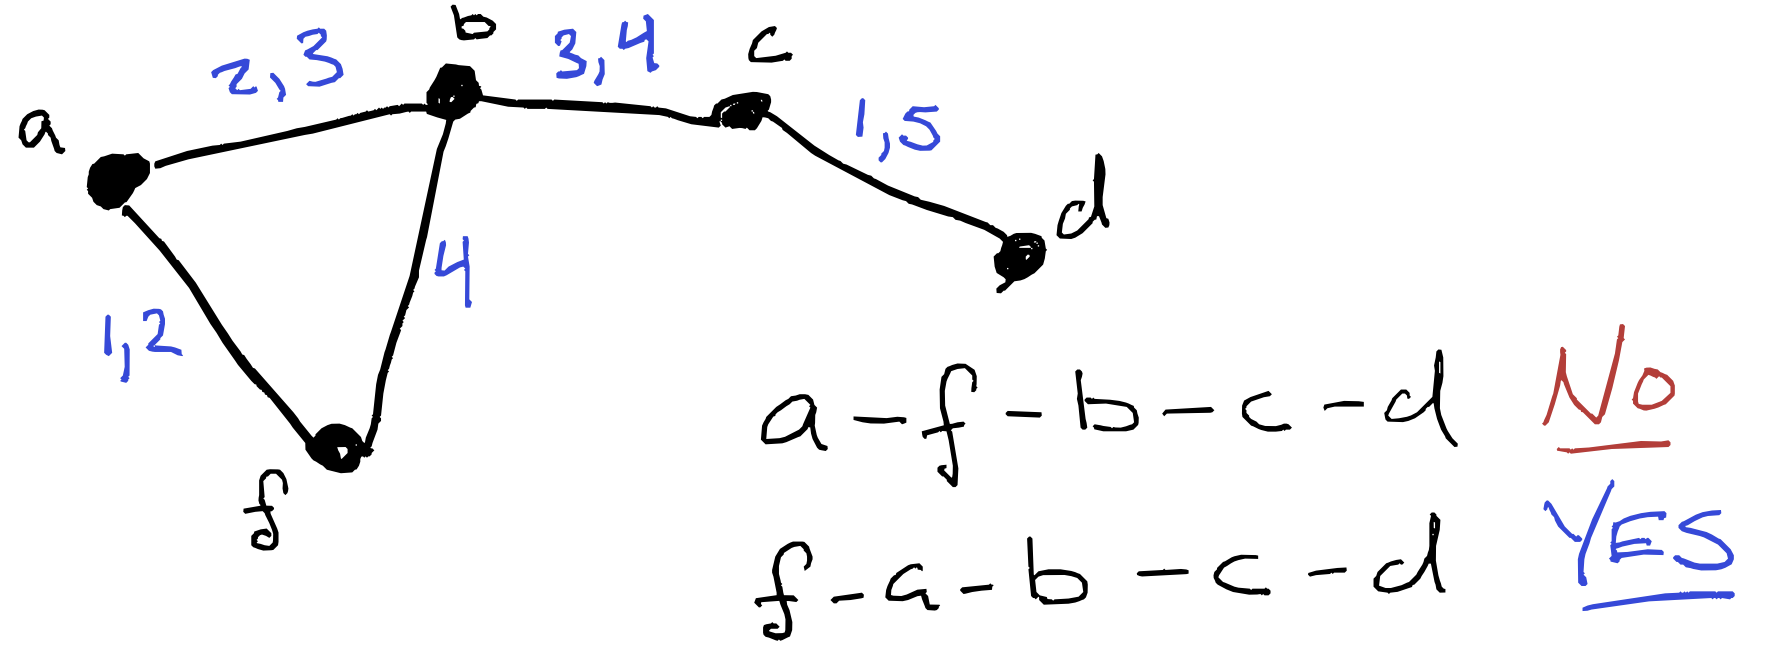
\includegraphics[width=1\linewidth]{temporal-hamiltonian-path.png}
\end{figure}

Is there a strict temporal path that visits every vertex exactly once?

\bigskip

This is of course hard from the static case.  


\end{frame}


\begin{frame}{Ex: Temporal Hamiltonian Path}
At a bag, a state must record which vertices are visited already, where the path ends so far. 

Key ingredients:
\begin{itemize}
\item we can generate all the states
\item we can check if a state is consistent with previous state
\item our state captures everything we need
\end{itemize}

% \begin{figure}
%     \centering
%     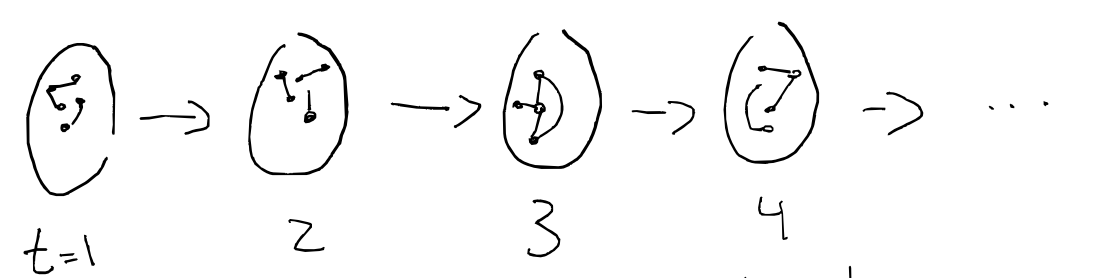
\includegraphics[width=0.75\linewidth]{vim-decomp.png}
% \end{figure}

\begin{figure}
    \centering
    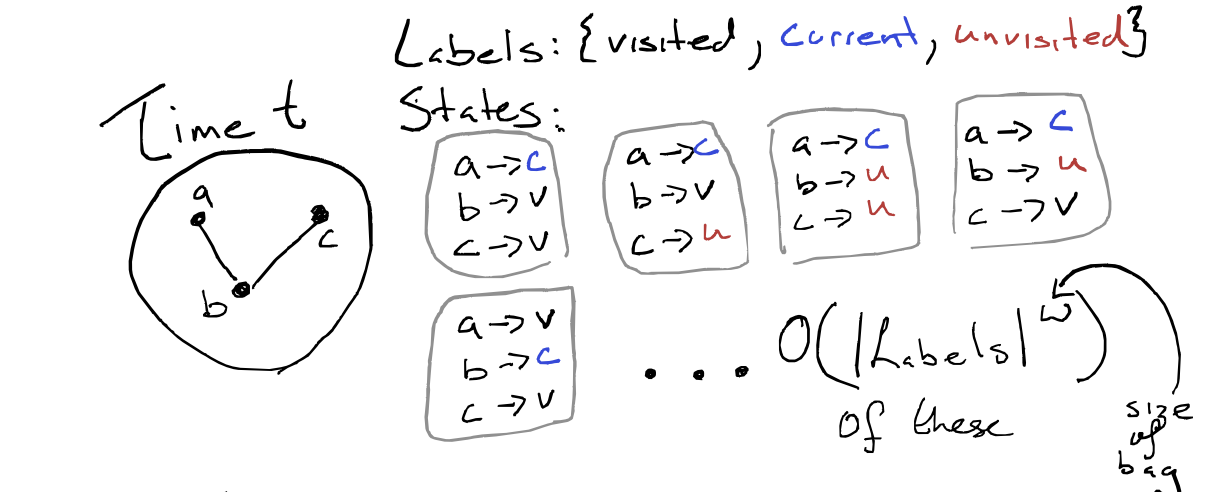
\includegraphics[width=0.75\linewidth]{smaller-decomp-ex.png}
\end{figure}


\end{frame}

\begin{frame}
\textbf{Much as I love these DPs they do start to feel a little similar.}

\bigskip

This has inspired a meta-algorithm that gives VIM DPs on a well-behaved type of problem.

\bigskip

What ingredients did we need?
\begin{itemize}
\item states that capture the problem, and we can ignore vertices outside their active interval
\item ability to generate starting states 
\item ability to check states from time to time
\item ability to check state at end-of-time to show we have solved problem
\end{itemize}

\end{frame}

% \begin{frame}{A bit more formal}
% We need a few escalating definitions:
% \begin{itemize}
% \item $(k, X)$-state
% \item $(k, X)$-temporally uniform problem
% \item $(k, X)$-locally temporally uniform problem
% \end{itemize}

% Punchline: If our problem is  $(k, X)$-locally temporally uniform, we can solve it using a VIM decomposition dynamic program in time:

% \bigskip

% $$
% O(\Lambda p(n)b^{2k}|X|^{2\omega})
% $$
% \begin{itemize}
% \item $\Lambda$ is the lifetime
% \item $p(n)$ is the time complexity of our checking and starting functions
% \item $b, k, X$ all have to do with the state
% \item $\omega$ is the VIM width
% \end{itemize}
% \end{frame}

% \begin{frame}{$(k, X)$-state}
% If we have:
% \begin{itemize}
% \item a set of labels $X$
% \item a natural number $k$
% \end{itemize}

% A $(k, X)$ state on a set of vertices $V$ is a pair $(\ell, c)$:
% \begin{itemize}
% \item $\ell$ maps vertices to labels
% \item $c$ is a vector of $k$ integers
% \end{itemize}

% \bigskip

% \textbf{Spoilers/Example:}\\
% For Temporal Hamiltonian Path 
% \begin{itemize}
% \item the labels will be \textcolor{red}{unvisited}, \textcolor{blue}{current}, visited
% \item the numbers will keep track of how many things we have visited    
% \end{itemize}



% \end{frame}

% \begin{frame}{$(k, X)$-temporally uniform}
% We require:
% \begin{itemize}
% \item $\exists$ a \texttt{transition} algorithm
% \item $\exists$ an \texttt{accepting} algorithm
% \item $\exists$ a set of starting states
% \end{itemize}
% such that an instance is a yes-instance iff
% \begin{itemize}
% \item $\exists$ a sequence of states over times that:
% \begin{itemize}
% \item starts in the set of starting states
% \item transitions one-to-the-next time, as verified by \texttt{transition} algorithm
% \item all states are accepted by \texttt{accepting} algorithm
% \end{itemize}
% \end{itemize}


% \end{frame}


% \begin{frame}{$(k, X)$-locally temporally uniform}

% We need all of the bits on the previous slide, plus:

% \begin{itemize}
% \item vertices can only change state at a time within active interval
% \end{itemize}
% (via a number of quite technical bits)

% \end{frame}

% \begin{frame}{What does the algorithm look like?}
% \begin{figure}
%     \centering
%     \includegraphics[width=1\linewidth]{example-dp-local.png}
% \end{figure}
% \end{frame}

% \begin{frame}{Temporal Hamiltonian Path}
% \begin{figure}
%     \centering
%     \includegraphics[width=0.95\linewidth]{hamiltonian-path-local-example.png}
% \end{figure}
% \end{frame}

\begin{frame}{But there's more!}
\redout{Tree Interval Membership} TIM width
\begin{figure}
    \centering
    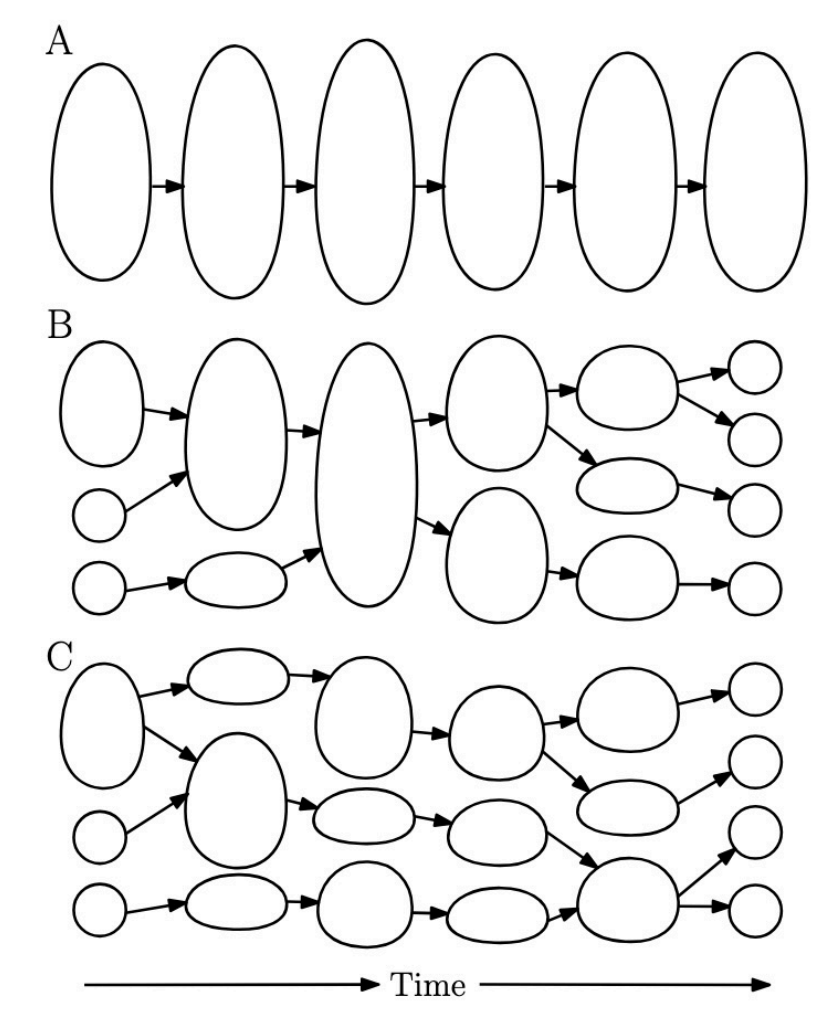
\includegraphics[width=0.3\linewidth]{all-the-widths.png}
\end{figure}

Here we need to be able to ignore not just vertices that are done being active or not yet active, but also ones that are in a different component in a particular way.

\end{frame}

% \begin{frame}
% \begin{figure}
%     \centering
%     \includegraphics[width=0.75\linewidth]{time-decom-example.png}
% \end{figure}
% \end{frame}


\begin{frame}{TIM is more complicated}
Sometimes TIM is more useful, sometimes VIM. 

\begin{tabular}{| c | c | c |}
 \hline
 \textbf{Problem} & \textbf{VIMW} & \textbf{TIMW} \\
 \hline
%  \textsc{Temporal Dominating Set}  & FPT  & FPT  \\
% \hline
\textsc{Temporal Hamiltonian Path}  & FPT  & FPT  \\
\hline
\textsc{$\Delta$-Temporal Matching}  & FPT  & FPT  \\
\hline
\textsc{Temporal Reachability Edge Deletion}  & FPT~[already known]  & FPT  \\
\hline
\textsc{Temporal Firefighter}  & FPT~[already known]  & NP-hard \\
\hline
\end{tabular}

\bigskip

\textbf{We have characterisations of problems that admit algorithms FPT by TIM and VIM by the requirements on those building blocks.}

\bigskip

These parameters are so helpful because they enforce sparseness: most vertices can be ignored most of the time.   

\end{frame}


\begin{frame}{We wanted parameters for `denser' temporal graphs}
We have started using a few generalisations from static parameters that allow lots of active edges at a time and give some tractability results.  
\begin{figure}
    \centering
    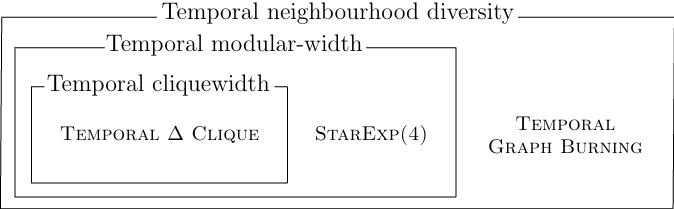
\includegraphics[width=0.9\linewidth]{target.png}
\end{figure}

\end{frame}

\begin{frame}{Neighbourhood diversity}

The \emph{neighbourhood diversity} of a graph $G = (V,E)$ is the smallest integer $k$ such that $V$ can be partitioned into sets $V_1,\dots,V_k$ with the property that, if $x,y \in V_i$ for any $i$ then $N(x)\setminus \{y\} = N(y)\setminus \{x\}$.
%Very restrictive -- number of numbers

\begin{center}


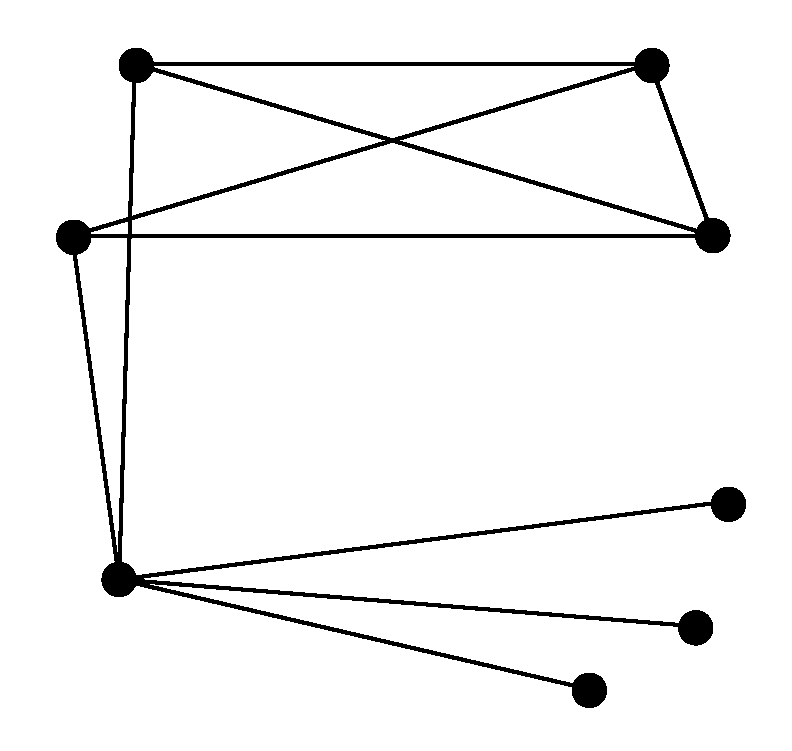
\includegraphics[width=0.5 \linewidth]{neighbourhood_diversity_graph}

\end{center}

\end{frame}
\begin{frame}{Neighbourhood diversity}

The \emph{neighbourhood diversity} of a graph $G = (V,E)$ is the smallest integer $k$ such that $V$ can be partitioned into sets $V_1,\dots,V_k$ with the property that, if $x,y \in V_i$ for any $i$ then $N(x)\setminus \{y\} = N(y)\setminus \{x\}$.
%Very restrictive -- number of numbers

\begin{center}

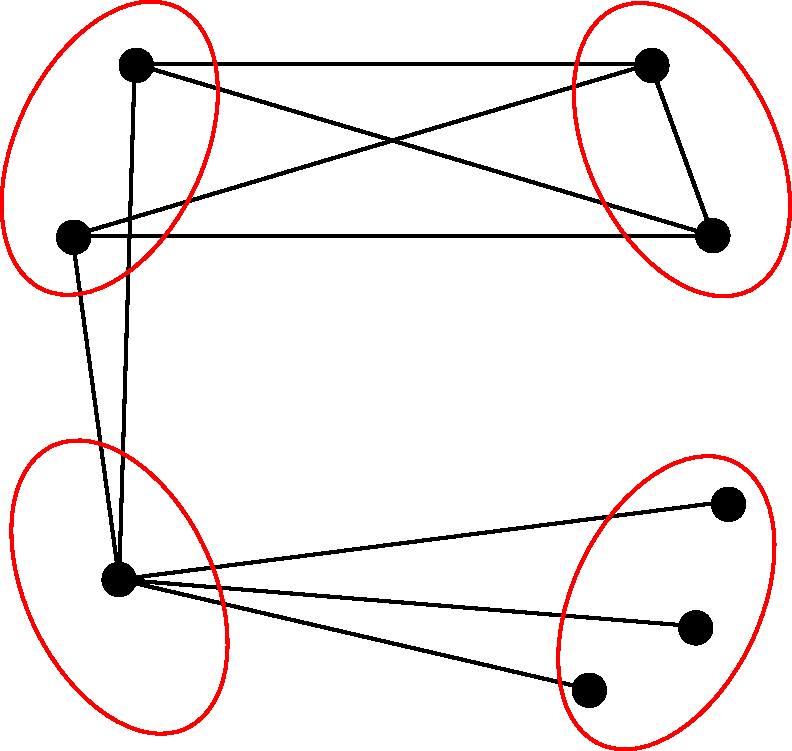
\includegraphics[width=0.5 \linewidth]{neighbourhood_diversity_decomp}


\end{center}

\end{frame}

\begin{frame}{Temporal Neighbourhood Diversity}

The \emph{temporal neighbourhood diversity} of a temporal graph $(G=(V,E),\lambda)$ is the smallest integer $k$ such that $V$ can be partitioned into sets $V_1,\dots,V_k$ with the property that, if $x,y \in V_i$ for any $i$ then, for all times $t$ and all vertices $z \notin \{x,y\}$, $t \in \lambda(xz)$ if and only if $t \in \lambda(yz)$.
%Very restrictive, but not number of numbers any more if the lifetime is large... also number of vertices considered reasonable parameter in this setting

\begin{center}

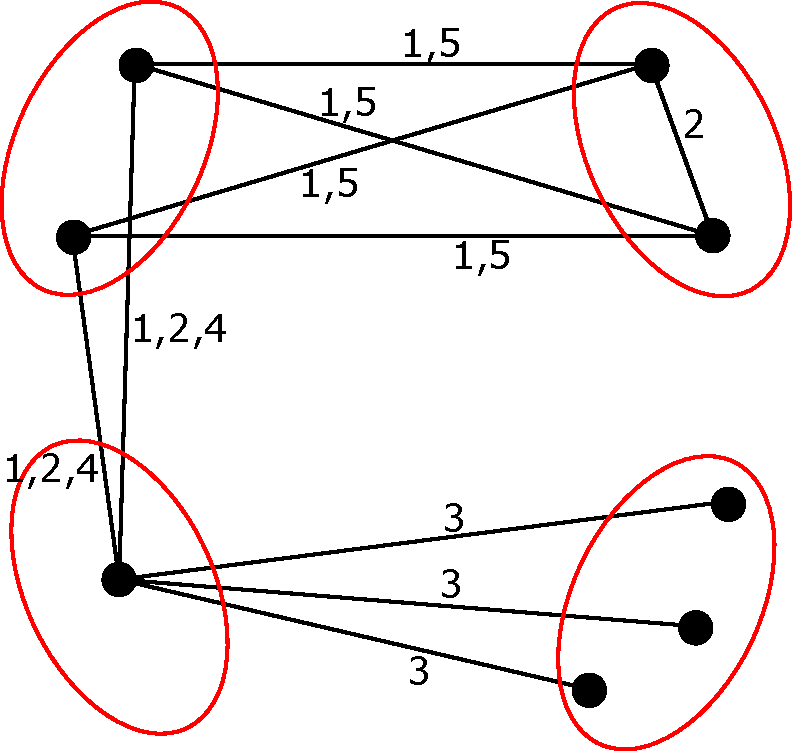
\includegraphics[width=0.5 \linewidth]{tnd_example}

\end{center}


\end{frame}
\begin{frame}{Temporal Neighbourhood Diversity}

The \emph{temporal neighbourhood diversity} of a temporal graph $(G=(V,E),\lambda)$ is the smallest integer $k$ such that $V$ can be partitioned into sets $V_1,\dots,V_k$ with the property that, if $x,y \in V_i$ for any $i$ then, for all times $t$ and all vertices $z \notin \{x,y\}$, $t \in \lambda(xz)$ if and only if $t \in \lambda(yz)$.
%Very restrictive, but not number of numbers any more if the lifetime is large... also number of vertices considered reasonable parameter in this setting

\begin{center}

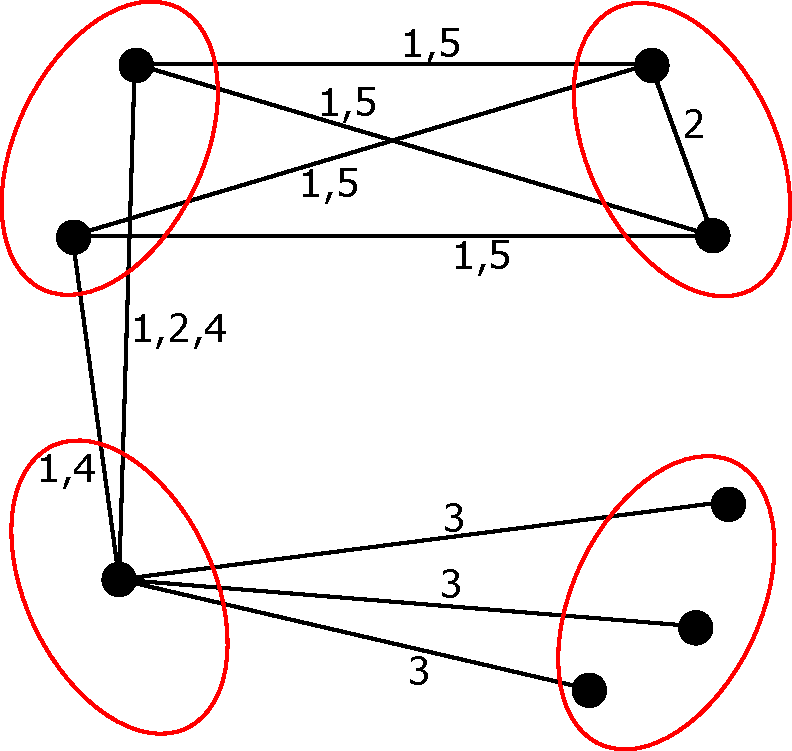
\includegraphics[width=0.5 \linewidth]{tnd_non-example}

\end{center}


\end{frame}


\begin{frame}{Tractability with temporal neighbourhood diversity}


Temporal Graph Burning:

\begin{enumerate}
    \item At time $t = 0$ a fire is placed at a chosen vertex. All other vertices are unburnt.
    \item At all times $t \geq 1$, the fire spreads, burning all vertices $u$ adjacent to an already burning vertex $v$ where the edge between $u$ and $v$ is active at time $t$. Then, another fire is placed at a chosen vertex.
    \item This process ends once all vertices are burning.
\end{enumerate}
\end{frame}

\begin{frame}{Tractability with temporal neighbourhood diversity}

\textsc{Temporal Graph Burning}\\
\textit{Input:} A temporal graph $(G, \lambda)$ and an integer $\ell$.\\
\textit{Question:} Does there exist a  successful burning strategy for $(G, \lambda)$ of length less than or equal to $\ell$?

\vspace{1cm}

\begin{theorem}
\textsc{Temporal Graph Burning} admits an FPT algorithm parameterised by the temporal neighbourhood diversity of the input graph.
\end{theorem}



\end{frame}

% \begin{frame}{Tractability with temporal neighbourhood diversity}

% % \only<1>{

% % \textsc{SingMinReachDelete}\\
% % \textit{Input:} A temporal graph $(G,\lambda)$, a vertex $s \in V(G)$ and  positive integers $k$ and $h$.\\
% % \textit{Question:} Is it possible to delete at most $k$ time-edges from $(G,\lambda)$ so that no more than $h$ vertices are reachable from $S$?

% % \vspace{0.5cm}

% % \begin{theorem}[Enright, Hand, Larios-Jones \& M., 2024+]
% % \textsc{SingMinReachDelete} is in FPT parameterised simultaneously by the temporal neighbourhood diversity of the input graph and the maximum number of appearances of any edge.
% % \end{theorem}

% % }

% \only<1-3>{

% \only<1>{
% Temporal Graph Burning:

% \begin{enumerate}
%     \item At time $t = 0$ a fire is placed at a chosen vertex. All other vertices are unburnt.
%     \item At all times $t \geq 1$, the fire spreads, burning all vertices $u$ adjacent to an already burning vertex $v$ where the edge between $u$ and $v$ is active at time $t$. Then, another fire is placed at a chosen vertex.
%     \item This process ends once all vertices are burning.
% \end{enumerate}

% \vspace{0.5cm}
% }

% \textsc{Temporal Graph Burning}\\
% \textit{Input:} A temporal graph $(G, \lambda)$ and an integer $\ell$.\\
% \textit{Question:} Does there exist a  successful burning strategy for $(G, \lambda)$ of length less than or equal to $\ell$?

% \only<2>{
% \vspace{1cm}

% \begin{theorem}
% \textsc{Temporal Graph Burning} admits an FPT algorithm parameterised by the temporal neighbourhood diversity of the input graph.
% \end{theorem}
% }

% }
% \end{frame}
\begin{frame}

\begin{figure}
    \centering
    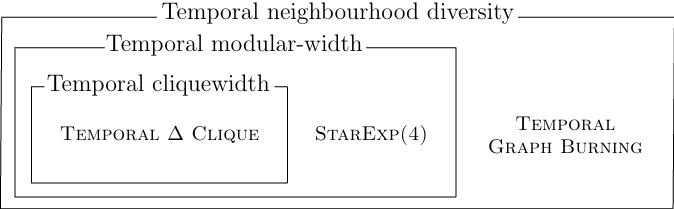
\includegraphics[width=0.9\linewidth]{target.png}
\end{figure}

\begin{conj}
Any temporal graph property expressible in first-order logic admits an FPT algorithm parameterised simultaneously by the temporal cliquewidth and the length of the formula.
\end{conj}

\end{frame}



% ===== begin extra comment
% \begin{frame}
% Modular-width can be thought of as the maximum degree in a modular (de)composition tree, where you make a graph with repeated joins and disjoint unions:

% \begin{figure}
%     \centering
%     \includegraphics[width=0.5\linewidth]{modular-decom-tree.png}
% \end{figure}
% \end{frame}


% \begin{frame}{Generalisation I: Temporal Modular Width}

% \only<1-6>{

% \begin{center}
% \only<1>{
% \includegraphics[width = 0.8 \linewidth]{MW_0}
% }
% \only<2>{
% \includegraphics[width = 0.8 \linewidth]{MW_1}
% }
% \only<3>{
% \includegraphics[width = 0.8 \linewidth]{MW_2}
% }
% \only<4>{
% \includegraphics[width = 0.8 \linewidth]{TMW_0}
% }
% \only<5>{
% \includegraphics[width = 0.8 \linewidth]{TMW_1}
% }
% \only<6>{
% \includegraphics[width = 0.8 \linewidth]{TMW_2}
% }
% \end{center}
% }


% \only<7-8>{

% \begin{theorem}
% \textsc{Temporal Graph Burning} is NP-hard even when restricted to graphs with constant temporal modular-width.
% \end{theorem}

% \vspace{1cm}

% \only<8>{
% \begin{theorem}
% \textsc{StarExp} is solvable in time $(k\tau)!(k\tau)^{O(1)}$ when the temporal modular-width of the graph is at most $k$ and every edge appears at most $\tau$ times.
% \end{theorem}
% }
% }
% %
% %Burning theorem
% %
% %StarExp theorem

% \end{frame}




% \begin{frame}{Generalisation II: Temporal Cliquewidth}

% \only<1-3>{
% \begin{itemize}
% \item Cliquewidth is a further generalisation of modular width, which allows an additional ``relabelling'' operation
% \item Graphs of bounded modular width cannot contain long induced paths, whereas an $n$-vertex path has cliquewidth 3 for arbitrarily large $n$
% \pause
% \item We define a natural temporal analogue as for the previous parameters
% \end{itemize}
% }

% \only<3>{
% \begin{theorem}
% \textsc{StarExp} is NP-hard on temporal graphs with temporal cliquewidth 3.
% \end{theorem}
% }

% \only<4>{

% \textsc{Temporal $\Delta$ Clique}\\
% \textit{Input:} A temporal graph $\mathcal{G}=(V,E,\lambda)$ and two integers $\Delta$ and $h$.\\
% \textit{Question:} Is there a set $V'\subseteq V$ of at least $r$ vertices such that, for every $u,v \in V'$ and every window of $\Delta$ consecutive timesteps, the edge $uv$ appears at least once in the window? 

% \vspace{0.5cm}

% \begin{theorem}
% \textsc{Temporal $\Delta$ Clique} is in FPT parameterised by the temporal cliquewidth of the input graph (provided that we are given a temporal cliquewidth construction of the input graph).
% \end{theorem}
% }

% \only<5>{


% \begin{frame}
% \begin{conj}
% Any temporal graph property expressible in first-order logic admits an FPT algorithm parameterised simultaneously by the temporal cliquewidth and the length of the formula.
% \end{conj}


% \end{frame}




\begin{frame}{Summary and Thanks!}
\textbf{In summary:\\}
There are a variety of approaches to parameters for temporal graphs.  Next up:

\begin{itemize}
\item Find more problems that are tractable parameterised by these parameters
% \pause
\vspace{0.5cm}
\item Is there a Courcelle-style metatheorem for temporal cliquewidth?
% \pause
\vspace{0.5cm}
\item Investigate the values of these parameters on real-world temporal networks 
\end{itemize}


\end{frame}


%% ===================================================================
%% Extra material: temporal c-closedness (shown after the thanks slide)
%% ===================================================================

\begin{frame}{Temporal c-closedness}
Now for something more inspired by the complex networks community.  

\bigskip

A temporal graph parameter that measures whether vertices that share neighbours over some small timespan are also themselves adjacent.



\bigskip
If a graph has low value of this parameter, and can't change too much from one time to the next, then we can efficiently enumerate its temporal cliques.

\bigskip

Some graphs from data have low-ish values for this parameter, or are close to doing so.




\end{frame}



% \section[Closure]{Triadic Closure and Temporal graphs}
\begin{frame}{$c$-closedness}
A static graph is $c$-closed if every pair of vertices that share at least $c$ neighbours are adjacent.

\begin{figure}
    \centering
    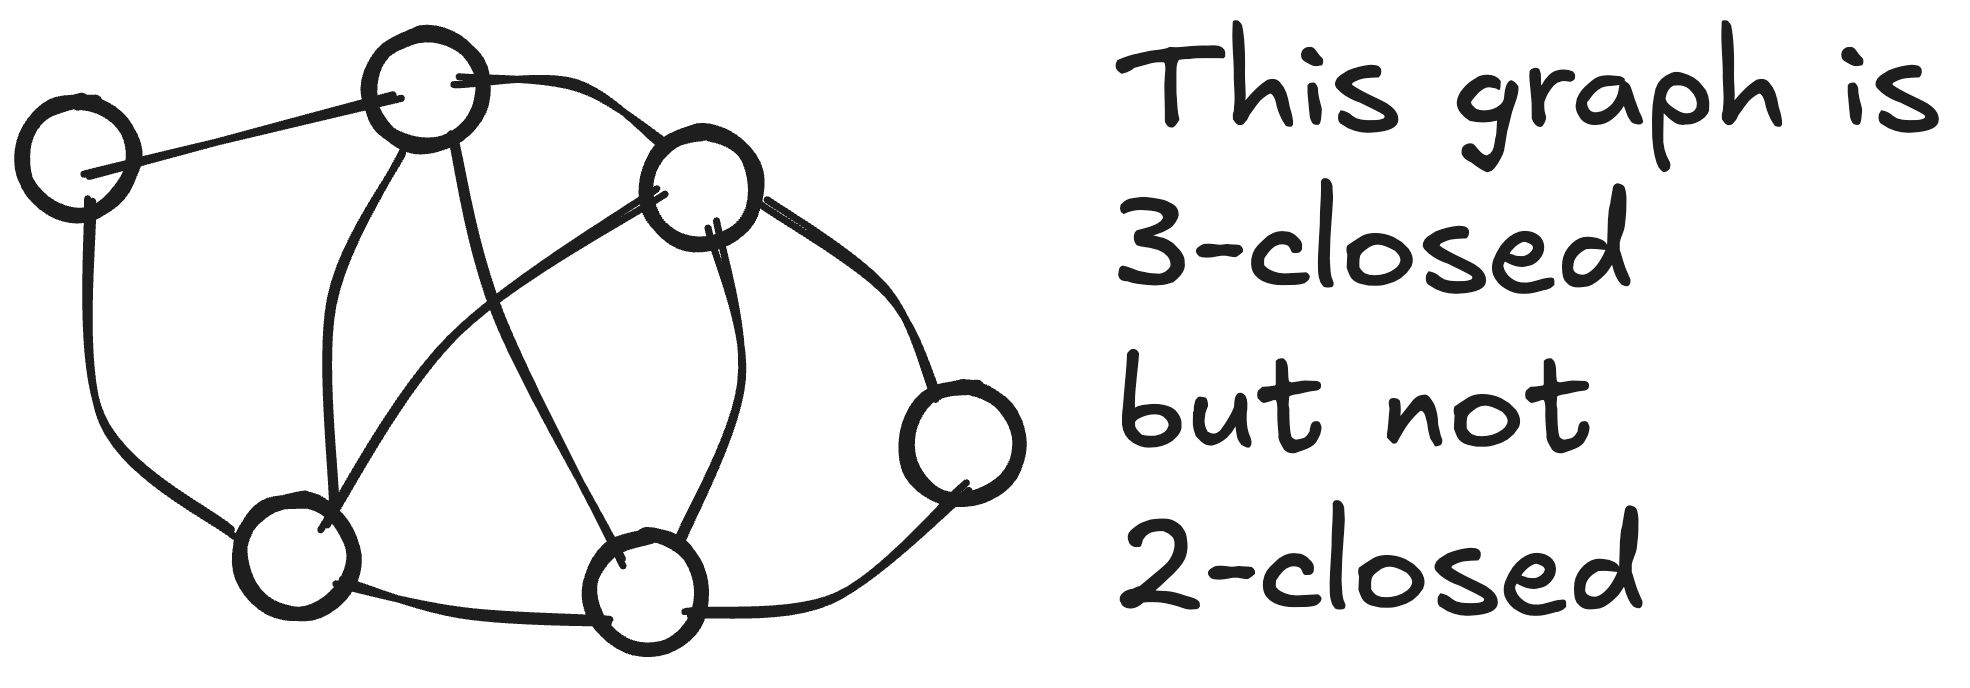
\includegraphics[width=0.75\linewidth]{static-closure.png}

\end{figure}
This bounds the number of maximal cliques, and helps with various algorithmic questions

\bigskip
\begin{figure}
    \centering
    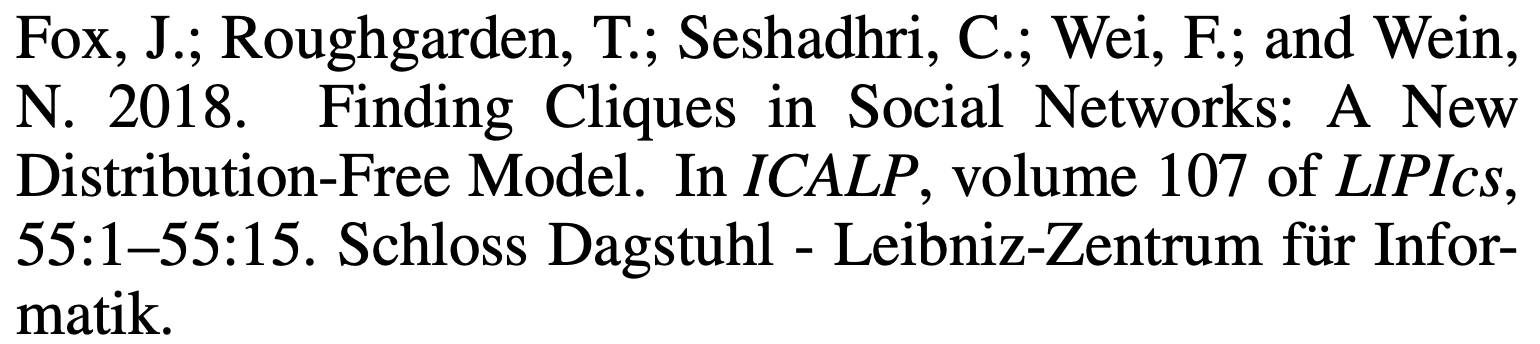
\includegraphics[width=0.4\linewidth]{citation.png}
\end{figure}


\end{frame}

\begin{frame}{What does this mean for a temporal graph?}
% a picture of a temporal graph
\begin{columns}
    \begin{column}{0.65\textwidth}
\textbf{What does it mean to share neighbours?}
\begin{itemize}
\item Ever?
\item In some time window?
\item Consistently?
\end{itemize}
\textbf{When would they then be adjacent?}
\begin{itemize}
\item Ever?
\item When they share neighbours?
\item After they share neighbours?
\item Before they share neighbours?
\item Always?
\end{itemize}
\end{column}
\begin{column}{0.4\textwidth}
\begin{figure}
    \centering
    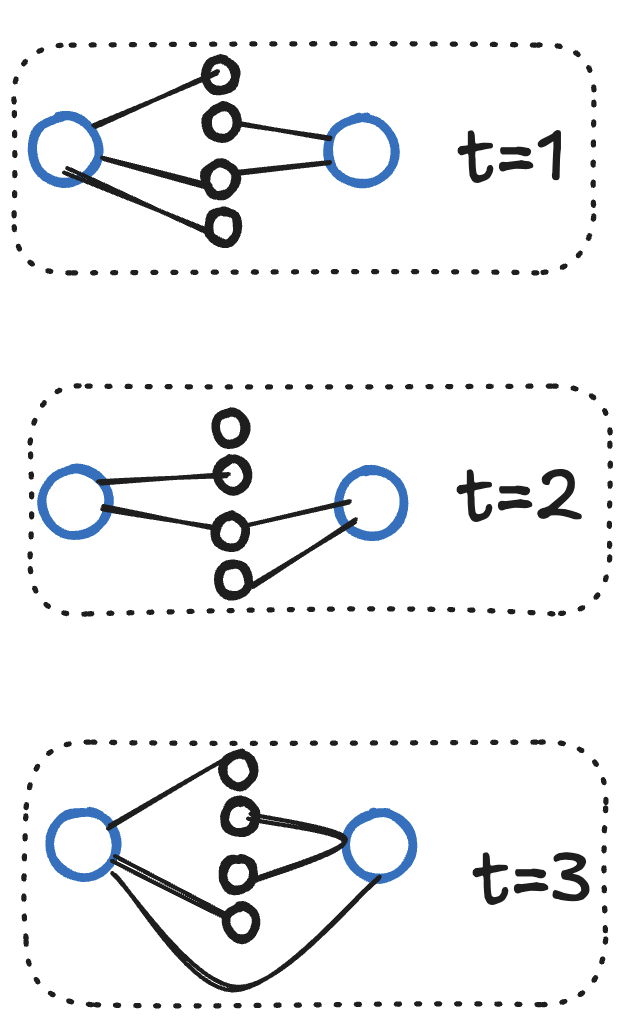
\includegraphics[width=1.0\linewidth]{example-temporal-triadic.png}
\end{figure}
\end{column}
\end{columns}
\end{frame}

\begin{frame}{We have picked a multi-parameter definition}
A temporal graph $(G, \lambda)$ is $(\Delta_0, \Delta_1, \Delta_2, c)$-closed when:

\begin{itemize}
    \item for every two distinct vertices $u, v \in V(G)$ and 
    \item any time-interval $[a, b]$ of length at most $\pone + 1$ (i.e., $b - a \leq \pone$) with $a \geq 1 + \pngt $ and $b \leq \lt_{\ca{G}} - \ptwo$,
\end{itemize}
if 
\begin{itemize}
    \item $u$ and $v$ have at least $c$ common neighbors during $[a, b]$,
\end{itemize}
then 
\begin{itemize}
    \item $u$ and $v$ are adjacent to each other during $[a - \pngt, b + \ptwo]$
\end{itemize}

  %   \begin{definition}[$(\pngt,\pone, \ptwo, c)$-closed graphs]\label{def:c-closed}
  % For integers $\pngt, \pone, \ptwo \geq 0$ and $ c \geq 1$, a temporal graph $\ca{G} = (G, \lambda)$ is $(\pngt, \pone, \ptwo, c)$-closed if the following condition holds: for every two distinct vertices $u, v \in V(G)$ and any time-interval $[a, b]$ of length at most $\pone + 1$ (i.e., $b - a \leq \pone$) with $a \geq 1 + \pngt $ and $b \leq \lt_{\ca{G}} - \ptwo$,  if $u$ and $v$ have at least $c$ common neighbors during $[a, b]$, then $u$ and $v$ are adjacent to each other during $[a - \pngt, b + \ptwo]$.  
% \end{definition}

\end{frame}

\begin{frame}
\begin{figure}
    \centering
    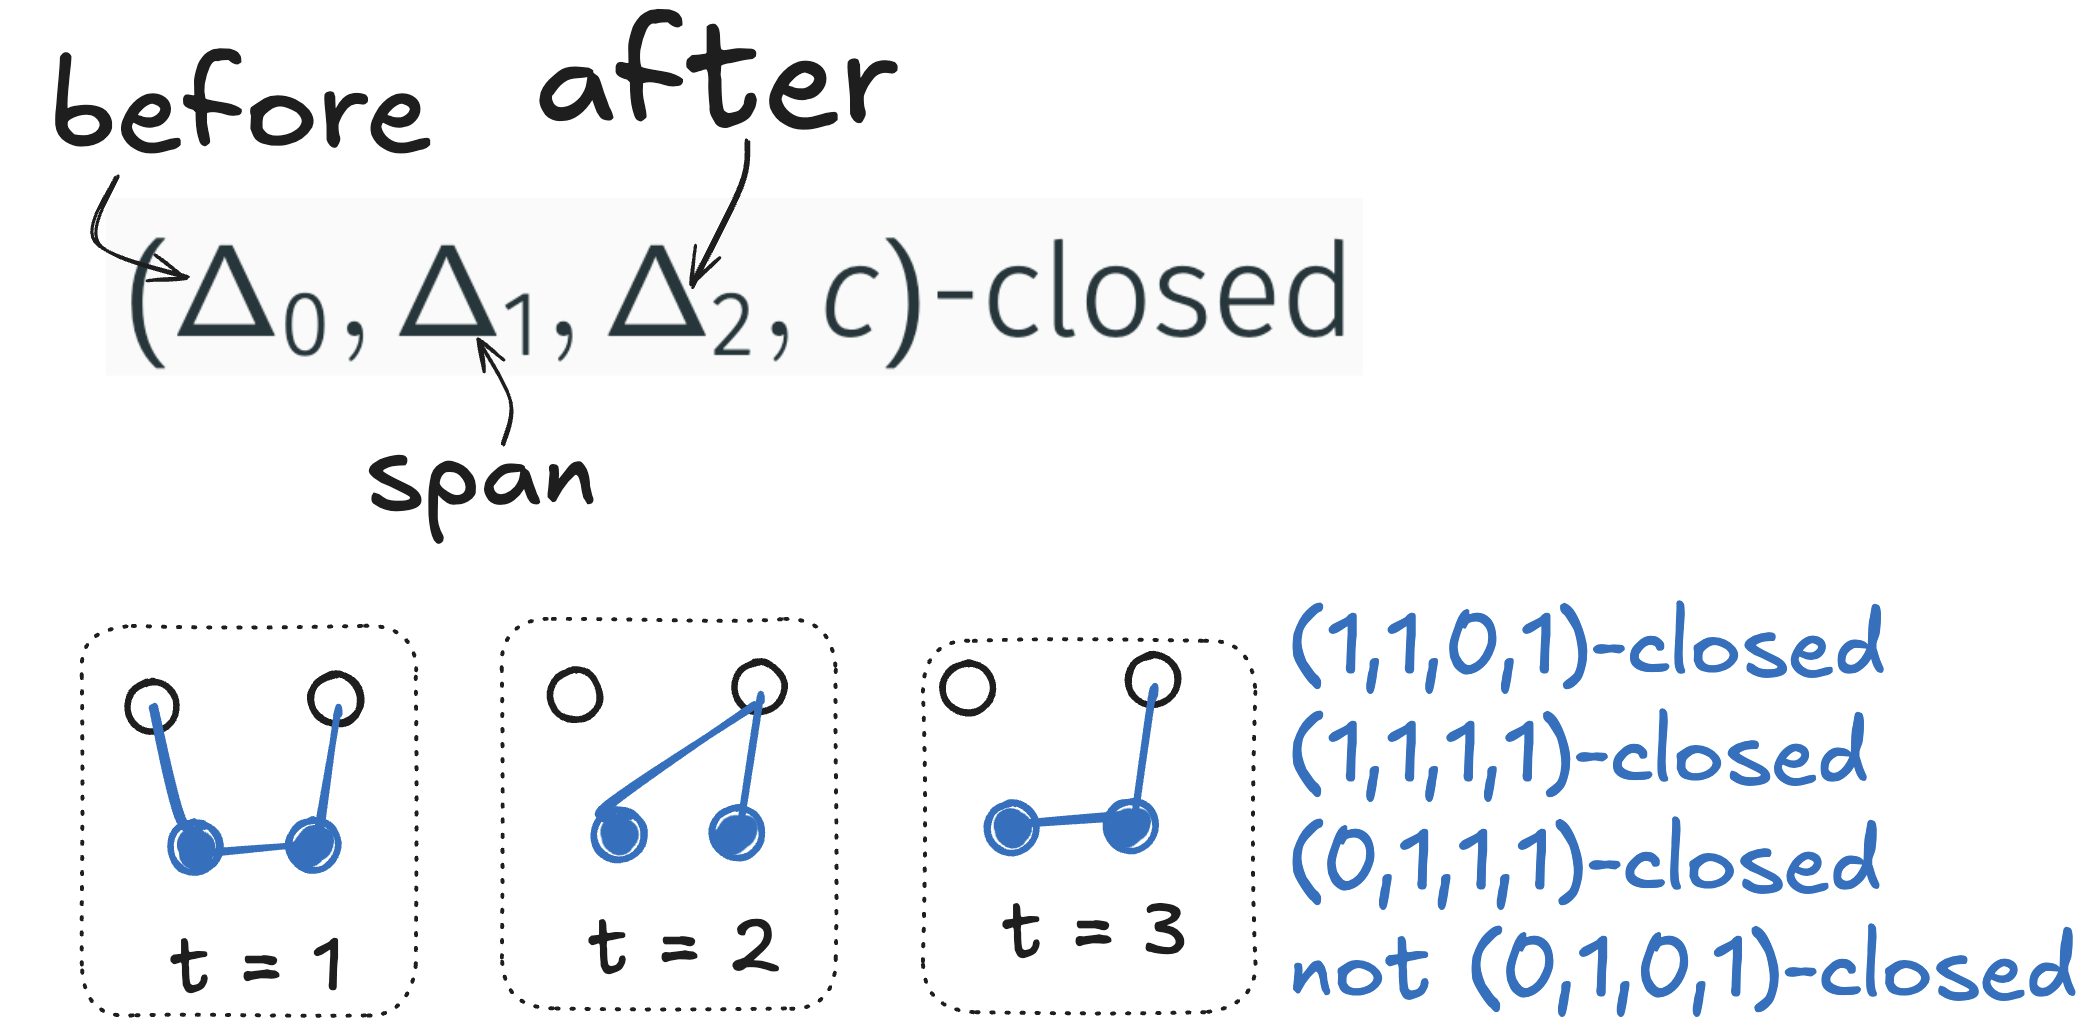
\includegraphics[width=1\linewidth]{example.png}
\end{figure}

The black vertices on top are not $(x,2,y,1)-$closed for any $x, y$
\end{frame}

% \section[Why]{What does this let you do?}
\begin{frame}{What does this let you do?}
In the static case, closure lets you enumerate maximal cliques efficiently.

\bigskip

That's our aim here, but we need something else to bound the number of maximal temporal cliques:

\bigskip

\textbf{local stability}

\end{frame}

\begin{frame}{But wait - we need more!}
\begin{definition}[locally $\eta$-unstable graphs]\label{def:eta-unstable}
    For a non-negative integer $\eta$, a temporal graph $\ca{G} = (G, \lambda)$ is locally $\eta$-unstable if $\max\set{\card{N_t(v) \setminus N_{t + 1}(v)}, \card{N_{t + 1}(v) \setminus N_{t}(v)}} \leq \eta$ for every vertex $v \in V(G)$ and every time-step $t \leq \lt - 1$. 
\end{definition}
\bigskip

 Intuition: neighbourhoods can change by at most $\eta$ vertices each time step. 

\end{frame}

\begin{frame}{I've lied to you slightly again...}
\textbf{DON'T READ THIS SLIDE. YOU DON"T WANT TO KNOW.}





\textcolor{yellow}{What we need is actually a little weaker than this - it's that the common neighbourhoods of vertices can't change too fast:}

\begin{definition}[pairwise $\eta$-unstable graphs]\label{def:pairwise-eta-unstable}
    \textcolor{yellow}{For a non-negative integer $\eta$, a temporal graph $\ca{G} = (G, \lambda)$ is pairwise  $\eta$-unstable if for any two distinct vertices $u$ and $v$ and any time-interval $[a, b]$  and non-negative integers $\ell, \ell'$ such that $[a - \ell, b + \ell'] \subseteq [1, \lt_{\ca{G}}]$, we have $\card{CN_{[a - \ell, b + \ell']}(u, v) \setminus CN_{[a, b]}(u, v)} \leq \eta (\ell + \ell')$.   }
\end{definition} 


\end{frame}

\begin{frame}
With all of this bounding machinery:

\bigskip

You can enumerate cliques efficiently parameterised by the triadic closure parameters plus the stability parameter:

\bigskip
{\huge $\mathcal{O}(2^{\weaknbdboundplus} \cdot n^2 \cdot m \cdot \lt)$} 

\bigskip

or

\bigskip

{\Large$\mathcal{O}($(exp in the params)(poly in input size)$)$}

\end{frame}

% \section[Data]{Does this reflect reality?}

\begin{frame}{Do data-derived graphs have these properties?}
How much does this occur in these particular graphs?
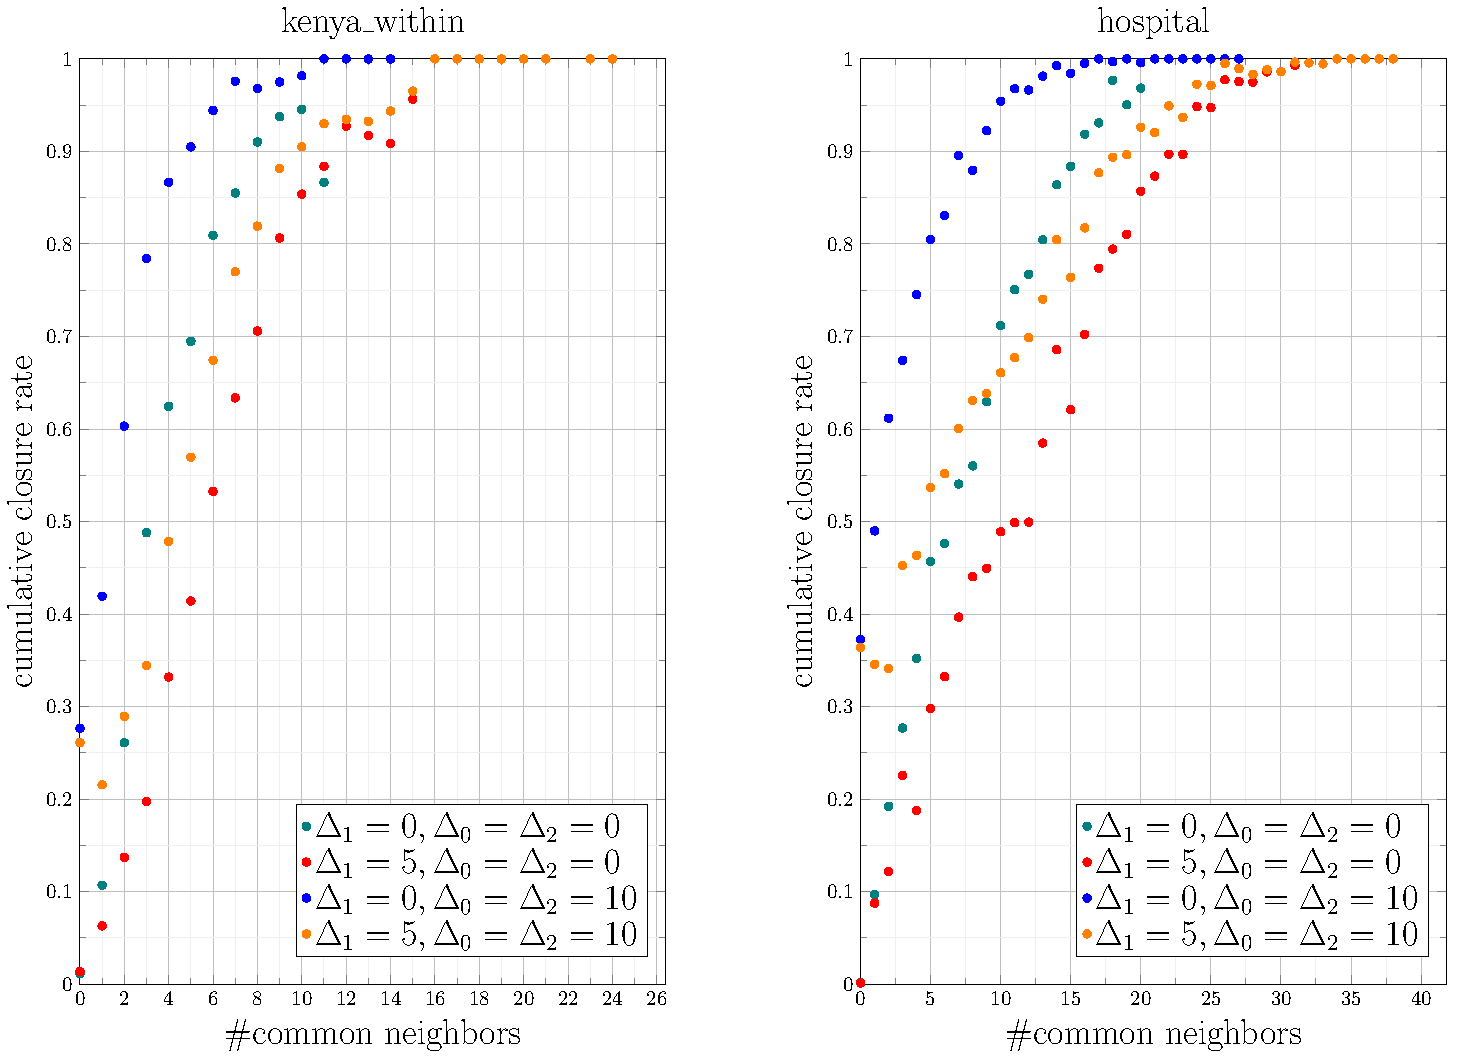
\includegraphics[width=0.8\linewidth]{cr-plots.pdf}

\end{frame}

\begin{frame}{Is this a useful set of parameters for data-derived temporal graphs?}
Somewhat.  

\bigskip

We looked at some SocioPatterns networks, and found that these parameters vary widely by network. 

\bigskip

For example, for two different workplace networks, we found:
\begin{itemize}
\item One with 95 nodes, instabilities in the 70s
\item One with 217 nodes, instabilities in the 20s
\end{itemize}

The picture is similar for closedness measures.

\begin{itemize}
\item When are these useful?
\item What is the right time step?
\item Where do these fit in the landscape of temporal graph parameters?
\end{itemize}


\end{frame}


\end{document}